\documentclass[conference]{IEEEtran}
\IEEEoverridecommandlockouts

\usepackage{amsmath,amssymb,amsfonts}
\usepackage{algorithmic}
\usepackage{graphicx}
\usepackage{textcomp}
\usepackage{xcolor}
\usepackage{biblatex}
\addbibresource{refs.bib}
\usepackage{subcaption}

\def\BibTeX{{\rm B\kern-.05em{\sc i\kern-.025em b}\kern-.08em
    T\kern-.1667em\lower.7ex\hbox{E}\kern-.125emX}}
    
\begin{document}

\title{BPC-PRP Project Documentation}

\author{\IEEEauthorblockN{Martin Kříž}
\IEEEauthorblockA{\textit{Department of Control and Instrumentation} \\
\textit{Brno University of Technology} \\
Brno, Czech Republic \\
246877@vut.cz}
\and
\IEEEauthorblockN{Filip Šlíma}
\IEEEauthorblockA{\textit{Department of Control and Instrumentation} \\
\textit{Brno University of Technology} \\
Brno, Czech Republic \\
247477@vut.cz}
}


\maketitle

\begin{abstract}
This work presents a set of control algorithms for the Fenrir mobile robot, designed to autonomously navigate and escape from a maze. The robot uses LiDAR, an IMU, wheel encoders, and a camera to perceive its environment. Navigation is managed by a finite state machine, featuring real-time line fitting for corridor detection, intersection classification, and IMU-based orientation correction and turning.
\end{abstract}

\begin{IEEEkeywords}
Autonomous robot, maze navigation, corridor following, ROS 2, LiDAR, IMU, ArUco tags
\end{IEEEkeywords}



\section{Introduction}
This paper presents the high-level control software for the mobile robot Fenrir, developed by the BUT robotics group for autonomous maze escape. The robot employs onboard sensors, including LiDAR, IMU, motor encoders, and a Raspberry Pi camera for detecting ArUco tags as navigation cues.

Built on ROS 2, the system interacts with low-level hardware via ROS topics and wirelessly communicates with a central PC for debugging. All modules are implemented as C++ ROS 2 nodes. Robot behavior is structured using a finite state machine governing tasks like corridor-following, turning, and IMU resetting \cite{fenrir_project}.



%\begin{figure}[h]
%    \centering
%    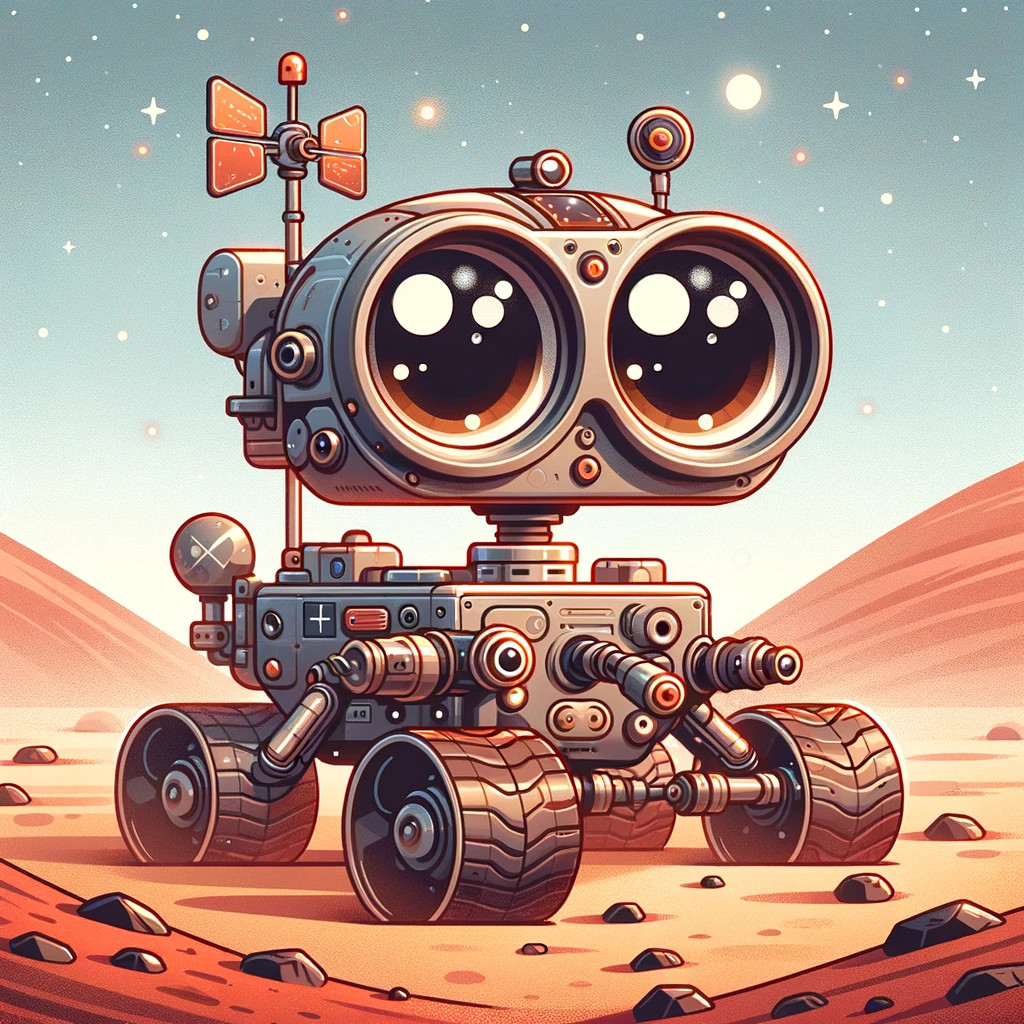
\includegraphics[width=0.45\textwidth]{images/rover.jpg}
%    \caption{The mars rover}
%    \label{fig:mars_rover}
%\end{figure}




\section{Main algorithms}
The robot’s high-level behavior during maze traversal is organized as a finite state machine, where each state corresponds to a distinct navigation task such as corridor following, turning, or intersection handling. The following sections describe the key algorithms used within these states.

\subsection{Line approximation from LiDAR data}
LiDAR data are collected in a polar format, with distance measurements sampled at regular angular increments. To extract meaningful structural information from the environment, the data are segmented into angular regions corresponding to different sectors around the robot. Within each sector, the points are approximated using a least-squares line-fitting algorithm. This is done in real time and allows the system to model walls or obstacles around the robot as straight lines. Multiple types of lines are fitted simultaneously, providing a more detailed representation of the environment. This approach enables the detection of walls that are perpendicular or parallel to the robot’s orientation, which can be used in maze where simple corridor assumptions may not hold. The example of the layout and interpretation of these fitted lines are illustrated in the figure \ref{fig:lidar_lines}. The output of this algorithm is a set of lines surrounding the robot, each expressed in the form \( y = kx + q \), where \( k \) represents the orientation of the line relative to the robot, and \( q \) denotes the perpendicular distance from the robot to the obstacle.

\subsection{Corridor following regulation}
Corridor driving is managed using front lines described in the previous section. A control mechanism evaluates the validity of these lines and selects the most reliable one to follow. If the robot is not centered within the corridor, the regulator aims to drive it back toward the middle. When the robot is already approximately centered (within a specified tolerance interval), the controller adjusts the robot's heading to remain parallel to the detected obstacle or wall.

\subsection{Intersection detection}
Intersection detection is categorized into two main types based on the presence of an obstacle directly in front of the robot. The first type includes intersections where the robot detects a wall upon entry — such as T-junctions with the stem facing forward, standard left or right turns, or dead ends. These require the robot to stop and make a decision about turning. The second type includes intersections where there is no obstacle directly ahead — such as left- or right-facing T-junctions and full X-crossings. This classification is essential for further processing. 

Intersection detection is also based on line approximations, as previously mentioned. However, it relies on lines fitted to more distant LiDAR regions than those used for corridor following. This allows the system to detect intersections early—before the corridor-handling algorithm might fail. The decision process evaluates the validity of the left and right line segments, along with the presence or absence of an obstacle in front of the robot. To suppress false positives caused by noise or transient sensor glitches, the intersection must be detected consistently at least three times before the robot reacts. If the condition is met less than three times, no behavioral change is triggered. Anyway, the detection is not entirely reliable, as the robot may not always approach intersections perfectly straight. This can lead to incorrect initial classification of the intersection type. Therefore, it is necessary to re-evaluate the intersection type during the handling process, in case the original detection was inaccurate.

\subsection{Intersection handling}
Intersections are handled based on the presence or absence of an obstacle in front of the robot. If a front obstacle is detected, the forward velocity controller drives the robot to a stop approximately 20 cm before the wall, ideally placing it at the center of the current cell.

The situation becomes more complex when there is no obstacle ahead. In this case, the robot attempts to reach the center of the cell using forward odometry calculated from wheel encoders. However, this method is inherently imprecise due to wheel slippage. Fortunately, since the distance is short, the resulting error is typically small and acceptable for practical purposes. The calculation of the forward odometry begins when a sudden change is detected in the left or right LiDAR points compared to the previous distances. This indicates that the robot has entered a new cell. After the robot reaches the center of the cell, a rotation is performed. The direction of the rotation is explained in the following text. The rotation is controlled by a regulator using feedback from the IMU to ensure accurate orientation.

\subsection{IMU setting and resetting}
Proper IMU calibration is a critical component of the navigation system. Without continuous correction, orientation drift could accumulate, potentially leading the robot to fail in exiting the maze due to additive angular error. The IMU is periodically reset during corridor following when the slope of the selected line is sufficiently low, indicating that the robot is aligned with the corridor. However, in some cases, this condition was not met quickly enough, and the reset did not occur in time, allowing error to accumulate. To address this, the system additionally performs an IMU correction after every turn. In this step, the algorithm selects the most parallel line and sets the robot's orientation angle using the formula: \(\varphi = \arctan(k)\) where \(k\) is the slope of the selected line.

\subsection{Turning strategy}
Based on ArUco tags detected by the onboard camera, the system stores the most recently observed markers. The hints are categorized separately for the treasure location and for the maze exit. If the robot encounters an intersection where one direction leads toward the treasure and the other toward the exit, the treasure is prioritized. However, if a hint for the exit has already been stored, it is recalculated and adjusted accordingly (e.g., if treasure $\rightarrow$ right and escape $\rightarrow$ left, then the robot turns right, then after the turn the directions are updated to treasure $\rightarrow$ unknown and escape $\rightarrow$ straight). This ensures that once the treasure is collected, the robot has an updated and valid direction for continuing toward the maze exit.

\subsection{State machine}
The state machine controls the robot's behavior while navigating a maze and consists of ten states. As shown in figure~\ref{fig:state_machine}, the initial state is calibration, which becomes active immediately after the program starts. In this state, the IMU sensor is calibrated, and once the calibration is complete, the robot transitions to the corridorFollowing state. This state is used to keep the robot centered in the corridor using data from the LIDAR and PID controllers. If an intersection with an obstacle directly ahead is detected, the state machine switches to the moveToTarget state, where the robot approaches the center of the intersection. If, on the other hand, an intersection without an obstacle ahead is detected, the coordinates are reset and the state transitions to resetCoordinates.

In the resetCoordinates state, the robot evaluates whether it has entered a new cell where a turn might be required. If so, it resets the coordinates again and transitions to the moveToCenterCoordinates state. If a new cell is not detected and the robot has already traveled more than 30 cm, it returns to the corridorFollowing state. In the moveToCenterCoordinates state, the robot moves toward the center of the cell, and it is checked whether there is an obstacle in front of the robot. If there is, the robot transitions back to the moveToTarget state. Once the robot reaches the center of the cell, it is verified whether it is at an intersection. If not, it returns to corridorFollowing. If it is at an intersection, it transitions to the getSpin state.

In the moveToTarget state, it is verified whether there is actually an obstacle in front of the robot. If no obstacle is detected, the robot returns to corridorFollowing. In this state, the robot moves to the center of the cell. Upon reaching the center, the LIDAR analyzes the surrounding walls, and based on their presence, the robot transitions to one of the states: turnLeft, turnRight, around, or, if both side walls are missing, to getSpin. In the getSpin state, information obtained via the camera and Aruco markers is used to determine the next state: turnLeft, turnRight, or littleGo, in the case the direction is straight.

The states turnLeft, turnRight, and around ensure the robot turns in the desired direction based on IMU data. Once the correct angle with a certain tolerance is reached, the robot transitions to the littleGo state. This state serves to move the robot approximately 10 cm forward to exit the intersection area, which allows it to correctly detect the corridor again and transition back to the corridorFollowing state.


\section{Conclusion}
This work presented navigation algorithms for the Fenrir robot, aimed at fast maze escape using LiDAR, IMU, encoders, and ArUco-based planning. Despite high-speed performance, some collisions occurred due to IMU drift and limited error handling. Future improvements include faster LiDAR sampling and moving control loops to a microcontroller for better precision.

\printbibliography

\section{Supplementary Materials}

\begin{figure*}[htbp]
  \centering
  \begin{subfigure}{\textwidth}
    \centering
    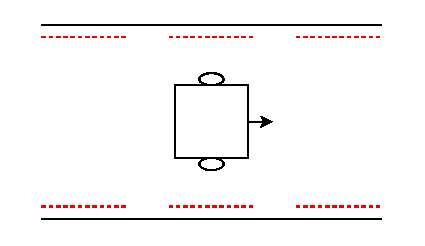
\includegraphics[width=0.6\textwidth]{images/PRP-lines.drawio.pdf}
    \caption{Example of lines around robot.}
    \label{fig:lidar_lines}
  \end{subfigure}

  \vspace{1em} % mezera mezi obrázky

  \begin{subfigure}{\textwidth}
    \centering
    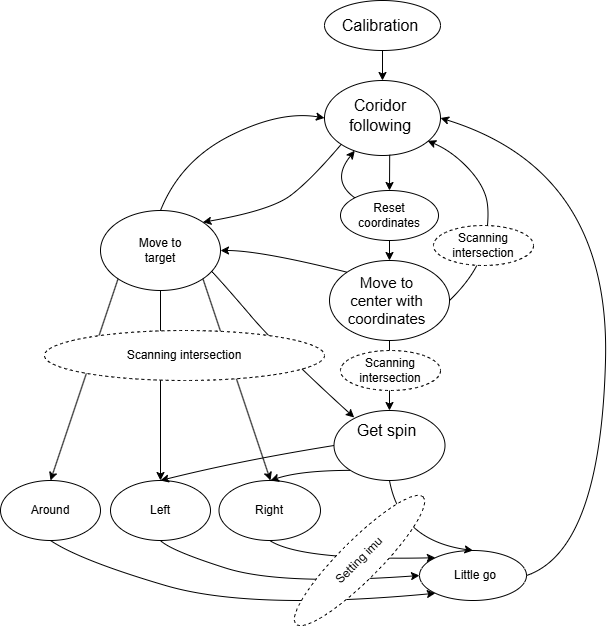
\includegraphics[width=0.6\textwidth]{images/PRP.drawio (1).png}
    \caption{State machine.}
    \label{fig:state_machine}
  \end{subfigure}
\end{figure*}



\end{document}
